% 02-methods.tex

% Section Title
\section{METHODS} \label{sec:methods}

    % In prose, describe the end-to-end procedure
    % - Devices and software: handset model, app, toolbox
    % - Data collection: where, how long, static vs. moving
    % - Spoofed-inputs: false position and delay parameters
    % - Optional interference scenario
    % - Processing: filtering criteria and solver workflow

    \subsection{Devices and Software}
    For this lab, we used a Samsung Galaxy A51 running Android 11. GNSS Logger v3.1.0.4 was chosen due to its comprehensive access to raw GNSS measurements, compatibility with recent Android APIs, and ability to log detailed GNSS data suitable for precision analysis. MATLAB R2024b was employed for data processing because it integrates Google's GNSS toolbox, facilitating robust analysis and visualization of GNSS measurements and position solutions.

    \subsection{Data Collection Procedure}
    Two distinct 5-minute GNSS data logging sessions were conducted on 3 May 2025, under cloudy weather conditions, using the GNSS Logger app configured with the following settings enabled:

    \begin{itemize}
        \item \textbf{GNSS Location:} Enabled to capture location data.
        \item \textbf{GNSS Measurements:} Enabled to log raw GNSS measurements.
        \item \textbf{Network Location:} Enabled to enhance location accuracy.
        \item \textbf{Navigation Messages:} Enabled to capture navigation data.
        \item \textbf{GnssStatus:} Enabled to log GNSS status information.
        \item \textbf{Sensors:} Enabled to capture sensor data.
    \end{itemize}
    The sessions were designed to capture both static and dynamic GNSS performance, with the following details:

    \begin{itemize}
        \item \textbf{Static Scenario:} Performed on the rooftop of Monte dei Cappuccini, Turin, starting at 10:35:20. The device was stationary throughout the entire session, providing baseline measurements.
        \item \textbf{Dynamic Scenario:} Conducted on tram line 15 from Piazza Castello to Piazza Vittorio Veneto, starting at 10:00:21, simulating a typical urban mobility scenario.
    \end{itemize}
    \begin{figure}[h!]
      \centering
      \begin{subfigure}{0.23\textwidth}
          \centering
          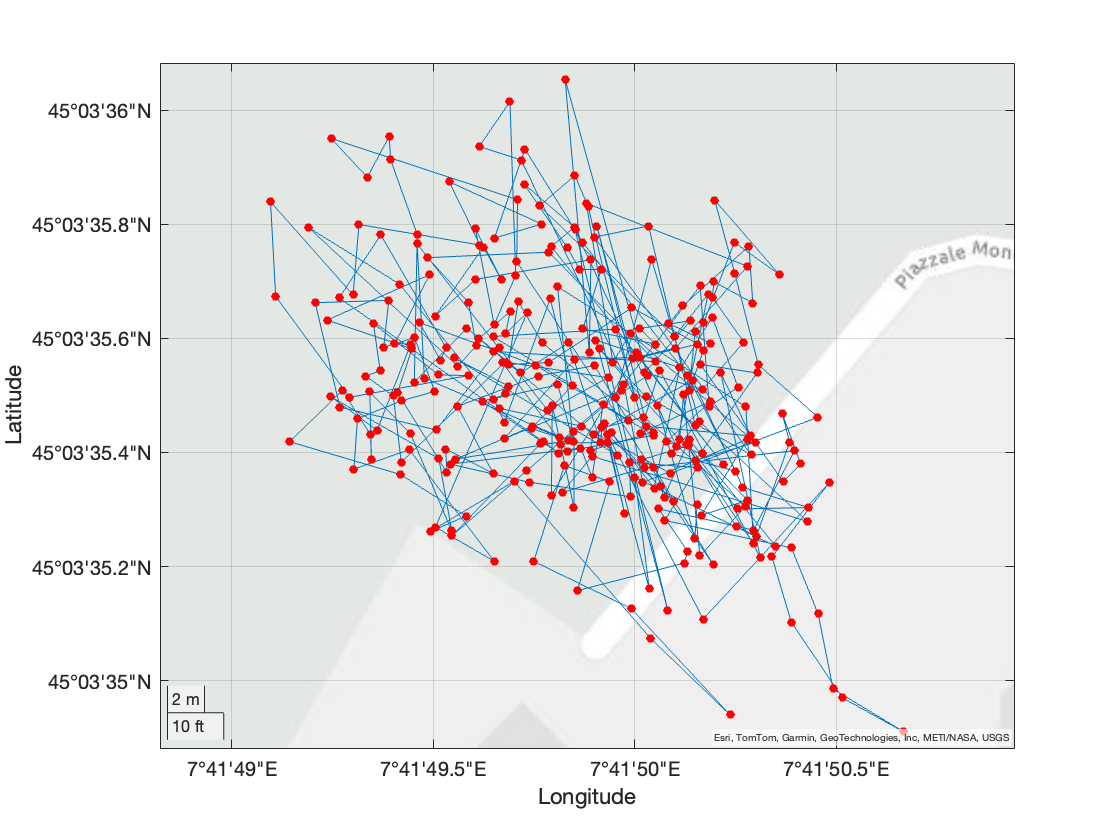
\includegraphics[width=\textwidth]{images/Monte_Cappuccini/filtered/Samsung_A51_Monte_Cappuccini_fig6.png}
          \caption{Monte dei Cappuccini.}
          \label{fig:static_scenario}
      \end{subfigure}
      \hfill
      \begin{subfigure}{0.23\textwidth}
          \centering
          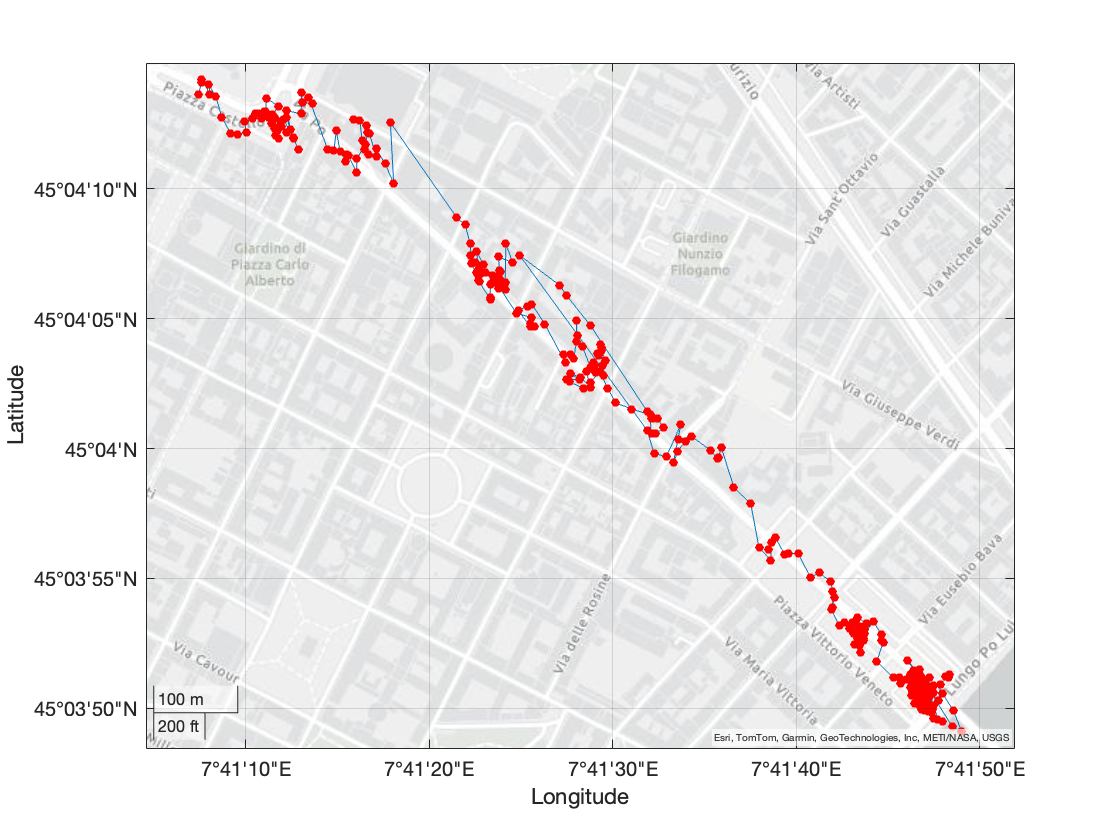
\includegraphics[width=\textwidth]{images/Tram_15_trip_Castello_to_Pescatore/filtered/Samsung_A51_Tram_15_trip_Castello_to_Pescatore_fig6.png}
          \caption{Tram Line 15.}
          \label{fig:dynamic_scenario}
      \end{subfigure}
      \vspace{0.35cm}
      \caption{Comparison of GNSS data: (a) Static scenario at Monte dei Cappuccini,(b) dynamic scenario along Tram Line 15.}
      \label{fig:gnss_comparison}
  \end{figure}

    \subsection{Processing Pipeline}
    The raw GNSS data from the GNSS Logger served as the input dataset for MATLAB. Processing involved a scripted workflow via \texttt{ProcessGnssMeasScript.m}, where the following steps were executed:
    \begin{enumerate}
        \item \textbf{Filtering:} Data points with a carrier-to-noise ratio below 25 dB-Hz or satellite elevations below 15° were excluded to improve accuracy.
        \item \textbf{Measurement Extraction:} Pseudorange and Doppler measurements were computed from GNSS timestamps and satellite transmission data.
        \item \textbf{Weighted Least Squares (WLS) Positioning:} Applied to derive precise positioning and clock bias estimates.
        \item \textbf{Visualization and Comparison:} Output plots from MATLAB, including pseudorange, pseudorange rates, and position solutions, were generated to facilitate comparative analysis of the static and dynamic scenarios.
    \end{enumerate}
    
    Results from this processing pipeline provided insights into the differences in GNSS performance under static and dynamic conditions.
    